\documentclass[conference]{IEEEtran}
\usepackage[utf8]{inputenc}
\usepackage[T1]{fontenc}
\usepackage[spanish,es-nodecimaldot]{babel}
\usepackage{graphicx,booktabs,amsmath,url}
\usepackage{cite}
\title{Prototipo de sombra digital para el monitoreo de una intersección vial en Paute, Ecuador}
\author{\IEEEauthorblockN{David Timbi y equipo}\IEEEauthorblockA{Proyecto académico, Paute, Ecuador}}
\begin{document}\maketitle
\begin{abstract}
Se presenta un prototipo de sombra digital para la intersección de la Av. Interoceánica (E40) y José Miguel Barzallo, en Paute, Ecuador. El sistema enlaza una cámara USB, detección de vehículos con YOLOv11, seguimiento de objetos, estimación de sentido y visualización 3D derivada de OpenStreetMap y SUMO. Un servidor local expone telemetría en tiempo real y una interfaz Three.js representa la escena. La exportación inspeccionada contiene 544 aristas, 231 junctions SUMO y 29 huellas de edificios; el punto de cámara usa el nodo 2910139955. Se describe el flujo de datos, la arquitectura y un protocolo de evaluación conforme a emparejamiento uno a uno. No se presentan cifras de precisión o desempeño de campo: al cierre de esta versión no se dispone de video anotado independiente ni protocolo de captura congelado. Por ello, los resultados se limitan a reproducibilidad del software, geometría y configuración del prototipo; las métricas empíricas quedan como trabajo pendiente.
\end{abstract}
\begin{IEEEkeywords}Sombra digital, tráfico, SUMO, YOLOv11, seguimiento, Paute.
\end{IEEEkeywords}
\section{Introducción}
La observación de tráfico mediante una cámara ofrece una señal directa del flujo local, mientras que un simulador microscópico permite explorar trayectorias y escenarios. La dificultad está en sincronizar ambas representaciones y distinguir observaciones reales de vehículos generados. Este trabajo construye una primera integración para el cruce de la E40 con José Miguel Barzallo, junto al Mercado 26 de Febrero. El objetivo es hacer explícito el ciclo datos--modelo--acción--medida--visualización y documentar qué evidencia existe hoy. El artefacto es un prototipo ejecutable, no una evaluación de precisión validada.

Las contribuciones son: (1) un puente local cámara--detector--interfaz 3D; (2) una referencia espacial única al junction SUMO 2910139955 y rutas etiquetadas SUBE/BAJA; y (3) un plan reproducible de evaluación que separa pruebas de lógica de datos de campo.
\section{Estado del arte}
Los sistemas de gemelo/sombra de tráfico integran flujos de datos con simulación para mantener una representación operativa; trabajos recientes estudian monitoreo y gestión en tiempo real a escala de red \cite{lu2025}. La literatura también destaca que la calibración microscópica debe contrastarse con trazas reales y que la plausibilidad de generación depende de los parámetros y composición vehicular \cite{calibration2021,ma2021,kusic2023}. Por tanto, una escena visual convincente no basta para demostrar fidelidad.

En detección y asociación, YOLOX documenta una arquitectura anchor-free con cabeza desacoplada y asignación SimOTA \cite{ge2021}; ByteTrack asocia también detecciones de baja confianza para reducir fragmentación de identidad \cite{zhang2022}. Ninguno garantiza desempeño en esta cámara: perspectiva, tamaño de buses, oclusión y movimiento rápido exigen validación local. Para posicionar cámaras en escenas 3D se han estudiado métodos imagen--nube de puntos, como TrafficLoc \cite{xia2025}; el prototipo actual no hace calibración visual 6-DoF: fija la cámara a un nodo de la red SUMO. Finalmente, conteos de sensores permanentes pueden ayudar a ajustar generación microscópica, pero no reemplazan el emparejamiento por vehículo \cite{probe2024}.

\begin{table*}[t]\centering\caption{Comparación de trabajos relacionados con el alcance del prototipo.}\label{tab:related}
\begin{tabular}{p{2.3cm}p{2.2cm}p{3.3cm}p{3.7cm}p{3.4cm}}\toprule
Trabajo & Año / contexto & Aporte & Evidencia que usa & Relación y diferencia\
\midrule
Ge et al. \cite{ge2021} & 2021, detección & Detector anchor-free YOLOX & COCO y benchmarks del artículo & Referencia de arquitectura; aquí se usa peso YOLOv11 preentrenado\
Zhang et al. \cite{zhang2022} & 2022, MOT & Asociación ByteTrack con cajas de baja confianza & MOT17/MOT20 & Se adopta configuración ByteTrack; falta medir ID switches localmente\
Kušić et al. \cite{kusic2023} & 2023, autopista & Sinergia de streams y simulación & Datos de dinámica vial en tiempo real & Motiva la integración; este prototipo es una sola intersección\
Ma et al. \cite{ma2021} & 2021, SUMO & Evalúa generación de flujo & Comparación de patrones de flujo & Informa la línea base sintética; no equivale a Ground Truth por objeto\
TrafficLoc \cite{xia2025} & ICCV 2025 & Localización 6-DoF de cámara & Imágenes y nubes de puntos & Aquí la pose se ancla por topología SUMO, sin estimación visual\
Lu et al. \cite{lu2025} & 2025, red vial & Herramienta de simulación gemela en tiempo real & Corrientes de detectores y simulación & Coincide en objetivo; el prototipo aún no evalúa gestión de red\
Conteos de sonda \cite{probe2024} & 2024, microsimulación & Conteos de sonda para detectores SUMO & Conteos y sensores automáticos & Sugiere calibración agregada; este informe requiere además matching individual\
\bottomrule\end{tabular}\end{table*}

\section{Metodología}
\subsection{Área y red}
La red se representa en SUMO y se exporta a JSON para Three.js. El artefacto actual indica 544 aristas, 231 junctions y 29 huellas de edificios. La referencia CCTV del JSON es el junction 2910139955, con ancla local $(11.87,0,-439.99)$, tramo 605329467\#6 y rutas dirigidas etiquetadas. La Fig. \ref{fig:network} muestra el entorno del punto de referencia; es una visualización derivada de la geometría, no un levantamiento topográfico independiente. OpenStreetMap aporta geometría base y requiere conservar atribución/licencia de sus datos.
\begin{figure}[t]\centering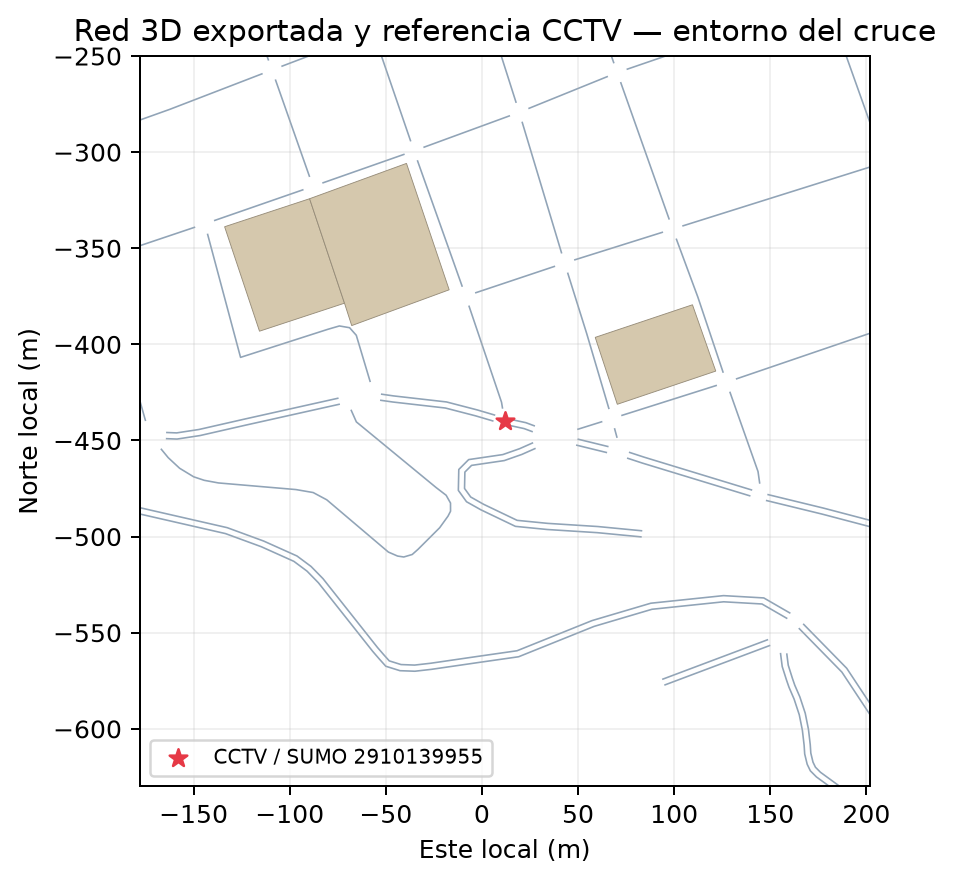
\includegraphics[width=\columnwidth]{figures/network_junction.png}\caption{Red vial y huellas exportadas alrededor del punto CCTV.}\label{fig:network}\end{figure}

\subsection{Cadena de observación}
El navegador entrega frames de la cámara USB al backend local; el detector identifica clases COCO relacionadas con vehículos y el tracker mantiene identidades entre frames. Una regla sobre el desplazamiento horizontal estima el sentido observado. La dirección está definida por el encuadre de cámara: SUBE corresponde a derecha--izquierda, BAJA a izquierda--derecha según el requisito operativo del proyecto. Los eventos de telemetría alimentan el HUD y las entidades de la escena. La Fig. \ref{fig:pipeline} resume el flujo. El servidor escucha por defecto HTTP en 8085 y el frontend se conecta a `/ws/telemetry`.
\begin{figure}[t]\centering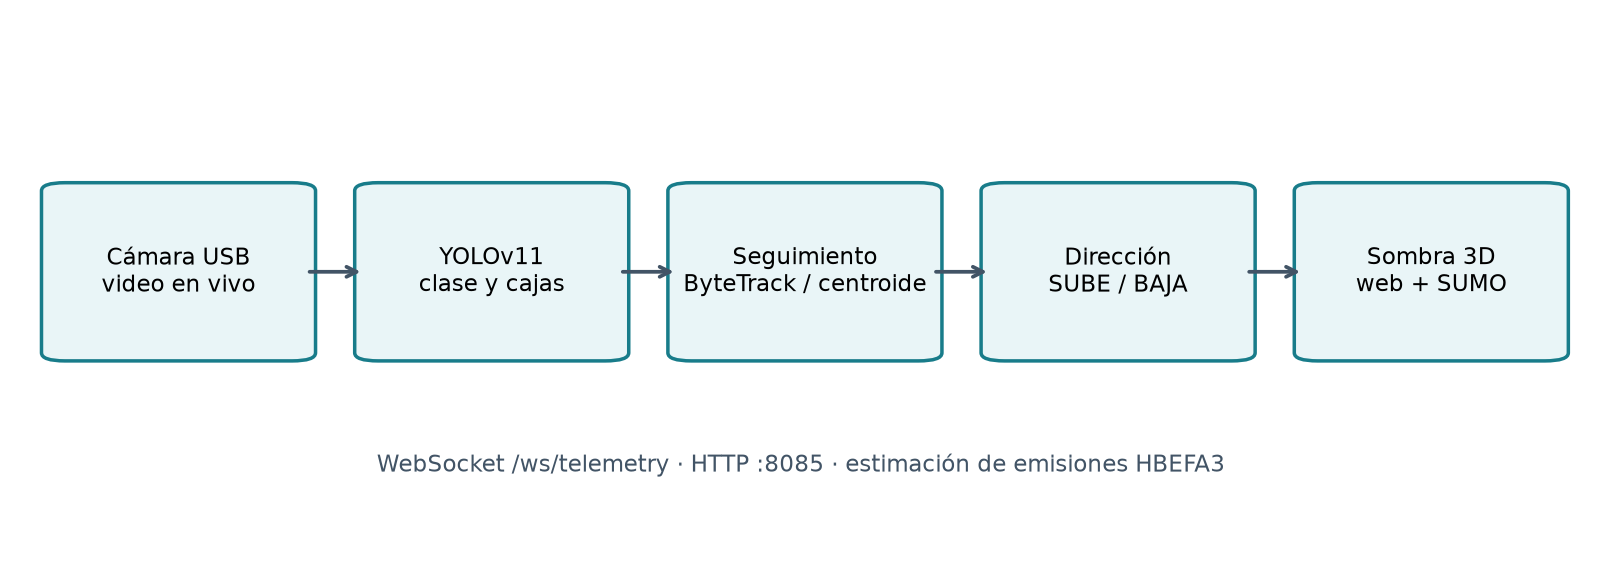
\includegraphics[width=\columnwidth]{figures/pipeline.png}\caption{Cadena implementada; CO$_2$ es una estimación configurada.}\label{fig:pipeline}\end{figure}

Se excluye tráfico sintético de SUMO en el radio de cámara para evitar que vehículos aleatorios se interpreten como detecciones. El sistema puede visualizar tráfico sintético fuera del área, pero éste debe identificarse como tal. La inyección de un evento detectado en una trayectoria simulada conectada es el objetivo del puente; no se afirma fidelidad de trayectoria hasta verificarlo con una traza sincronizada. El CO$_2$ se calcula con factores configurados inspirados en HBEFA3 y parámetros de flota, no con sensores de emisiones.

\subsection{Protocolo de evaluación propuesto}
Sea $R$ el conjunto anotado de cruces de referencia y $S$ el conjunto de eventos emitidos por la sombra. Una asignación bipartita uno a uno minimiza una función de coste de diferencia temporal y aproximación espacial, restringida al mismo intervalo de aproximación. Si $M$ son pares válidos, $P=|M|/|S|$ y $R_c=|M|/|R|$; deben reportarse además $|M|$, fantasmas $|S|-|M|$ y omisiones $|R|-|M|$. Exactitud de clase se calcula sobre pares $M$; sentido correcto sobre pares con referencia direccional. El retraso firmado es $t_S-t_R$ en la línea de conteo. Error de posición solo se calcula si se calibran coordenadas imagen--suelo. El archivo `validation/annotations_template.csv` define columnas iniciales; aún no hay anotaciones llenas.

\section{Implementación y reproducibilidad}
El código está organizado en `scripts/`, `web/`, `config/`, `net/` y `data/`. El servidor usa Python y bibliotecas declaradas en `requirements.txt`; el frontend sirve la visualización Three.js. La configuración SUMO registra semilla 42 y paso 0.1 s; TraCI usa puerto 8813 cuando SUMO está activo. El modelo `yolo11n.pt` no se incluye en el repositorio, por tamaño/licencia y porque debe obtenerse desde su fuente oficial aceptando sus términos. La red exportada y la escena se regeneran con `python scripts/export_network_3d.py`.

Para reproducir: registrar commit/tag, SO, Python, `pip freeze`, versión SUMO, peso exacto/hash, configuración, semilla, cámara y condiciones de captura; generar la red y ejecutar el servidor. La versión de la red indica que fue construida con SUMO 1.18.0; las versiones instaladas deben registrarse por cada ejecución. El repositorio no guarda videos ni salidas XML grandes. El protocolo no puede regenerar métricas de campo hasta que se agreguen videos autorizados y etiquetas de referencia. El sistema actual carece de un modo offline de reproducción acelerada con búsqueda, considerado una mejora pendiente.

\section{Resultados disponibles y discusión}
La inspección reproducible del JSON confirma 544 aristas, 231 junctions, 10 POI y 29 polígonos de edificios, además de una referencia CCTV con rutas SUBE/BAJA. La interfaz incorpora cámara, HUD y vista 3D; el backend declara YOLOv11, seguimiento y eventos direccionales. La configuración de ByteTrack usa `track_buffer=60` y `match_thresh=0.85`. Estos son resultados de inspección de artefacto/configuración, no medidas de calidad de detección.

El proyecto se encuentra en etapa de prototipo. No existe un conjunto de referencia anotado que permita afirmar recall, precisión, exactitud de clase, identificación de sentido, error espacial o demora. Tampoco hay una comparación cuantitativa contra un baseline SUMO calibrado. Las pruebas sintéticas de lógica sirven para detectar regresiones de reglas, pero no validan la robustez ante motos pequeñas, buses que ocupan gran parte del cuadro, oclusiones, sombras o vehículos estacionados. Se debe declarar el número de minutos anotados, conteos por clase/sentido, criterios de matching y exclusiones al presentar resultados futuros.

Las principales limitaciones son: pose de cámara fijada por topología y no calibración fotogramétrica; dependencia de iluminación y perspectiva; clases del detector genéricas que no separan necesariamente sedán de pickup; factores de emisiones aproximados; y trazabilidad todavía por consolidar con una etiqueta Git remota. La diferencia entre la clase visual y subtipos locales (p.ej. camioneta frente a sedán) exige una taxonomía y una matriz de confusión propia.

\section{Conclusiones y trabajo futuro}
Se integró una primera sombra visual para un cruce identificado de Paute, con geometría vial/edificada, punto CCTV explícito y canal de telemetría local. La documentación distingue la operación observable de la validación todavía no realizada. El siguiente paso científico es capturar un intervalo autorizado, anotar independientemente vehículos y sentidos, congelar la configuración, ejecutar matching uno a uno y publicar conteos con denominadores. Después se deben medir demora, clase, trayectoria y emisiones modeladas; añadir reproducción offline y comprobar que la entidad inyectada sigue una ruta conectada correspondiente al sentido observado. Hasta entonces, los resultados no deben interpretarse como precisión de campo.

\section*{Agradecimientos y datos}
La cartografía base proviene de OpenStreetMap; conservar atribución y verificar ODbL al redistribuir extractos. El escenario y el código son artefactos del proyecto académico. No se incorpora video de personas o vehículos.
\bibliographystyle{IEEEtran}
\bibliography{referencias}
\end{document}
